% Preamble
\documentclass[11pt]{PyRollDocs}
\usepackage{textcomp}

% Document
\begin{document}

    \title{The Wusatowski Spreading PyRoll Plugin}
    \author{Max Weiner}
    \date{\today}

    \maketitle

    This plugin provides a spreading modelling approach with Wusatowski's formula for flat rolling, adapted on groove rolling by an equivalent rectangle approach.


    \section{Model approach}\label{sec:model-approach}

    \subsection{Wusatowski's spread equation}\label{subsec:wusatowski's-spread-equation}

    Wusatowski proposed the \autoref{eq:wusatowski} for estimation of spreading in flat rolling,
    where $\gamma = \frac{h_1}{h_0}$ is the compression. $h$ and $b$ are height and width of the workpiece with the indices
    0 and 1 denoting the incoming respectively the outgoing profile. $a$, $c$, $d$ and $f$ are correction
    coefficients for temperature, velocity, material and friction, respectively.

    \begin{equation}
        \beta = \frac{b_1}{b_0} = a \times c \times d \times f \times \gamma^{-w}
        \label{eq:wusatowski}
    \end{equation}

    \noindent The velocity coefficient $c$ can be assumed as below in dependence on the velocity $v$.

    \begin{equation}
        c = \left(-0.002958 + 0.00341 \gamma \right) v + 1.07168 - 0.10431 \gamma
        \label{eq:velocity-coefficient}
    \end{equation}

    $w$ is the spread exponent, many different expressions were given by various authors for its value.
    The original expression by Wusatowski is given in \autoref{eq:exponent}, where $R$ is the roll radius.

    \begin{equation}
        w = 10^{ \num{-1.269} \left( \frac{h_0}{2 R} \right)^{\num{0.56}} \frac{b_0}{h_0} }
        \label{eq:exponent}
    \end{equation}

    \subsection{Equivalent rectangle approach}\label{subsec:equivalent-rectangle-approach}

    Wusatowskis spreading model was originally built for flat rolling.
    A common approach for groove rolling is to calculate some equivalent rectangular profile to be able to use flat rolling models.
    \autoref{fig:equivalent_rectangle} shows 3 variants of calculating an equivalent rectangle of a profile.

    \begin{figure}
        \centering
        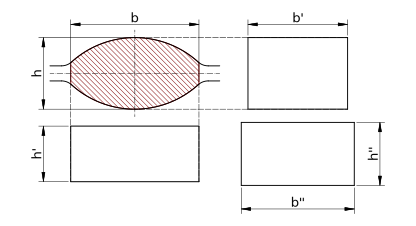
\includegraphics[width=\linewidth]{equivalent_rectangle}
        \caption{Three methods of defining an equivalent rectangle of an oval groove}
        \label{fig:equivalent_rectangle}
    \end{figure}

    The first variant is to keep the width constant and calculate the height $h'$ so that the cross section $A$ is
    equal:

    \[
        h' = \frac{A}{b}
    \]

    The second variant is to keep the height constant and calculate the width $b'$ so that the cross section $A$ is
    equal:

    \[
        b' = \frac{A}{h}
    \]

    Both represent the geometry of the profile poorly.
    A better way is to keep the aspect ratio equal:

    \[
        h'' = \sqrt{\frac{A h}{b}}
    \]

    \[
        b'' = \sqrt{\frac{A b}{h}}
    \]

    This variant is used in the current implementation.
    So $h$ and $b$ in Wusatowski's model are replaced with $h''$ and $b''$.
    In the end, $b_1$ can be obtained from $b_1''$ by:

    \[
        b_1 = \frac{b_1'' h_1}{h_1''}
    \]


    \section{Usage instructions}\label{sec:usage-instructions}

    The plugin can be loaded under the name \texttt{pyroll\_wusatowski\_spreading}.

    An implementation of the \lstinline{width_change} hook on \lstinline{RollPass} is provided,
    calculating the spread using the equivalent rectangle approach and Wusatowski's model.

    Several additional hooks on \lstinline{RollPass} are defined, which are used in spread calculation, as listed in \autoref{tab:hookspecs}.
    Base implementations of them are provided, so it should work out of the box.
    For \lstinline{wusatowski_exponent} and \lstinline{wusatowski_velocity_coefficient} the equations~\ref{eq:exponent} and~\ref{eq:velocity-coefficient} are implemented.
    The others default to \num{1}.
    Provide your own hook implementations or set attributes on the \lstinline{RollPass} instances to alter the spreading behavior.

    \begin{table}
        \centering
        \caption{Hooks specified by this plugin. Symbols as in \autoref{eq:wusatowski}.}
        \label{tab:hookspecs}
        \begin{tabular}{ll}
            \toprule
            Hook name                                     & Meaning                                \\
            \midrule
            \texttt{wusatowski\_temperature\_coefficient} & temperature correction coefficient $a$ \\
            \texttt{wusatowski\_velocity\_coefficient}    & velocity correction coefficient $c$    \\
            \texttt{wusatowski\_material\_coefficient}    & material correction coefficient $d$    \\
            \texttt{wusatowski\_friction\_coefficient}    & friction correction coefficient $f$    \\
            \texttt{wusatowski\_exponent}                 & spread exponent $w$                    \\
            \bottomrule
        \end{tabular}
    \end{table}

\end{document}